\documentclass[12pt,letterpaper]{article}

% --- Packages ---
\usepackage[margin=1in]{geometry}
\usepackage{titlesec}
\usepackage{hyperref}
\usepackage{graphicx}
\usepackage{listings}
\usepackage{xcolor}
\usepackage{enumitem}
\usepackage{booktabs}
\usepackage{fancyhdr}
\usepackage{float}
\usepackage{caption}
\usepackage{tikz}
\usetikzlibrary{shapes.geometric, arrows.meta, positioning, fit, calc}

% --- Colors ---
\definecolor{codeblue}{RGB}{0,70,127}
\definecolor{codegray}{RGB}{128,128,128}
\definecolor{codebg}{RGB}{248,248,248}
\definecolor{framecolor}{RGB}{180,180,180}

% --- Code listing style ---
\lstdefinestyle{cstyle}{
  backgroundcolor=\color{codebg},
  commentstyle=\color{codegray}\itshape,
  keywordstyle=\color{codeblue}\bfseries,
  stringstyle=\color{teal},
  basicstyle=\ttfamily\small,
  breaklines=true,
  captionpos=b,
  frame=single,
  rulecolor=\color{framecolor},
  tabsize=2,
  language=C
}

% --- TikZ styles ---
\tikzset{
  block/.style={rectangle, draw, rounded corners=4pt, fill=blue!8,
                text width=3.2cm, align=center, minimum height=0.8cm, font=\small},
  smallblock/.style={rectangle, draw, rounded corners=4pt, fill=blue!8,
                text width=2.4cm, align=center, minimum height=0.7cm, font=\small},
  dbblock/.style={cylinder, draw, shape aspect=0.3, fill=yellow!15,
                  text width=2.2cm, align=center, font=\small},
  decision/.style={diamond, draw, fill=orange!15, aspect=2,
                   align=center, font=\small},
  arrow/.style={-Stealth, thick},
  dasharrow/.style={-Stealth, dashed, thick}
}

% --- Header / footer ---
\pagestyle{fancy}
\fancyhf{}
\rhead{GroupChat Design Document}
\lhead{Operating Systems Final Project}
\cfoot{\thepage}

% --- Section formatting ---
\titleformat{\section}{\large\bfseries}{}{0em}{\thesection\quad}
\titleformat{\subsection}{\normalsize\bfseries}{}{0em}{\thesubsection\quad}

% ============================================================
\begin{document}

\begin{titlepage}
  \centering
  \vspace*{2cm}
  {\Huge\bfseries GroupChat\par}
  \vspace{0.5cm}
  {\Large Design Document\par}
  \vspace{0.3cm}
  {\large Operating Systems Final Project\par}
  \vspace{2cm}
  \rule{0.6\textwidth}{0.4pt}\\[0.4cm]

  % Hand-drawn sketch
  \begin{figure}[H]
    \centering
    
\includegraphics[width=0.65\textwidth]{IMG_1986.PNG}
    \caption{Initial hand-drawn architecture sketch: Client $\leftrightarrow$ Protocol $\leftrightarrow$ Server
             with audio, text, and image message types.}
  \end{figure}

  \vfill
  {\large May 5, 2026\par}
\end{titlepage}

\tableofcontents
\newpage

% ============================================================
\section{Architecture Overview}

\subsection{System Summary}

GroupChat uses a client-server model over TCP.
Multiple clients connect to one central server. The server owns group membership
state, routes chat/media traffic, and enforces scheduling decisions for
text-message processing.

\medskip
\noindent\textbf{Core responsibilities:}
\begin{itemize}[leftmargin=1.5em]
  \item \textbf{Client:} user command parsing, local media file I/O, frame send/receive, playback.
  \item \textbf{Server accept loop:} accepts sockets and creates one reader thread per client.
  \item \textbf{Server thread pool:} executes queued text tasks using RR (FIFO) or SJF.
  \item \textbf{Group manager:} tracks group membership, caches recent messages, handles synchronization.
  \item \textbf{Shared protocol layer:} frame parsing/encoding and constants.
\end{itemize}

\subsection{Client-Server Design Diagram}

\begin{figure}[H]
\centering
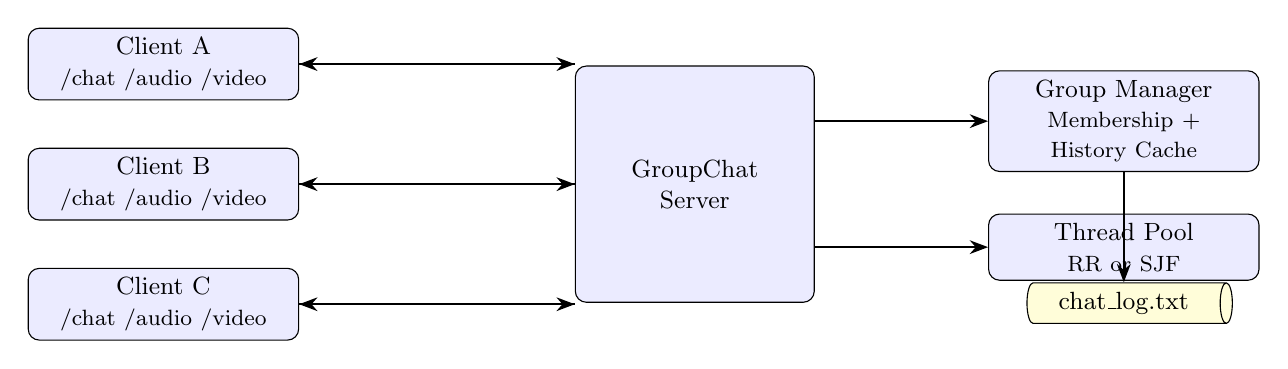
\begin{tikzpicture}[node distance=1.8cm and 2.6cm]
  % Clients
  \node[block] (c1) {Client A\\{\footnotesize /chat /audio /video}};
  \node[block, below=0.6cm of c1] (c2) {Client B\\{\footnotesize /chat /audio /video}};
  \node[block, below=0.6cm of c2] (c3) {Client C\\{\footnotesize /chat /audio /video}};

  % Server
  \node[block, right=3.5cm of c2, minimum height=3cm, text width=2.8cm] (srv) {GroupChat\\Server};

  % Sub-nodes below server
  \node[block, right=2.2cm of srv, yshift=0.8cm] (gm)
        {Group Manager\\{\footnotesize Membership + History Cache}};
  \node[block, right=2.2cm of srv, yshift=-0.8cm] (tp)
        {Thread Pool\\{\footnotesize RR or SJF}};
  \node[dbblock, below=1.4cm of gm] (log) {chat\_log.txt};

  % Arrows clients -> server
  \draw[arrow] (c1.east) -- (srv.west |- c1.east);
  \draw[arrow] (c2.east) -- (srv.west);
  \draw[arrow] (c3.east) -- (srv.west |- c3.east);

  % Arrows server -> sub-nodes
  \draw[arrow] (srv.east |- gm) -- (gm.west);
  \draw[arrow] (srv.east |- tp) -- (tp.west);
  \draw[arrow] (gm.south) -- (log.north);

  % Arrows server -> clients
  \draw[dasharrow] (srv.west |- c1.east) -- (c1.east);
  \draw[dasharrow] (srv.west) -- (c2.east);
  \draw[dasharrow] (srv.west |- c3.east) -- (c3.east);
\end{tikzpicture}
\caption{Client-server overview. Dashed arrows indicate messages broadcast back to clients.}
\end{figure}

\subsection{Server Thread Model (Including Thread Pool)}

The server has two levels of concurrency:

\begin{itemize}[leftmargin=1.5em]
  \item \textbf{Level 1 (I/O reader threads):} one thread per connected client reads incoming frames.
  \item \textbf{Level 2 (worker pool):} a fixed-size worker pool executes text-message tasks from
        a shared dispatch queue.
\end{itemize}

\medskip
\noindent\textbf{Design intent:}
\begin{itemize}[leftmargin=1.5em]
  \item I/O remains responsive for many clients.
  \item CPU-style task scheduling policy can be demonstrated and measured independently (RR/SJF).
  \item Shared mutable state is isolated in \texttt{GroupManager} and guarded by a mutex.
\end{itemize}

\begin{figure}[H]
\centering
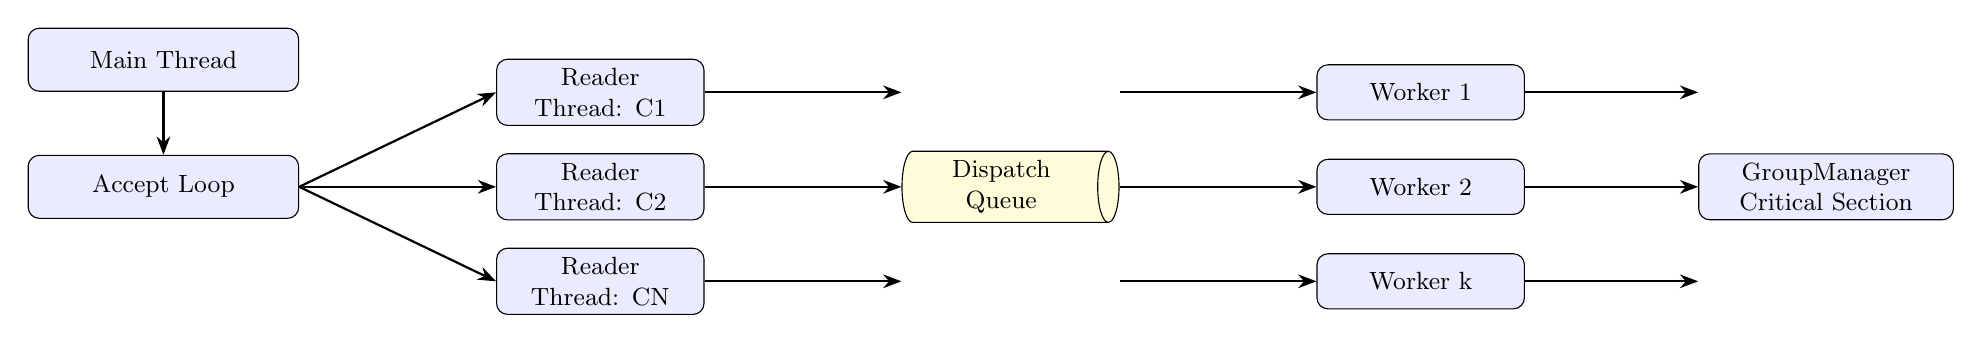
\begin{tikzpicture}[node distance=0.8cm and 2.0cm]
  % Main thread
  \node[block] (main) {Main Thread};
  \node[block, below=of main] (accept) {Accept Loop};
  \draw[arrow] (main) -- (accept);

  % Reader threads
  \node[smallblock, right=2.5cm of accept, yshift=1.2cm] (r1) {Reader\\Thread: C1};
  \node[smallblock, right=2.5cm of accept] (r2) {Reader\\Thread: C2};
  \node[smallblock, right=2.5cm of accept, yshift=-1.2cm] (rn) {Reader\\Thread: CN};

  \draw[arrow] (accept.east) -- (r1.west);
  \draw[arrow] (accept.east) -- (r2.west);
  \draw[arrow] (accept.east) -- (rn.west);

  % Queue
  \node[dbblock, right=2.5cm of r2] (queue) {Dispatch\\Queue};
  \draw[arrow] (r1.east) -- (queue.west |- r1.east);
  \draw[arrow] (r2.east) -- (queue.west);
  \draw[arrow] (rn.east) -- (queue.west |- rn.east);

  % Workers
  \node[smallblock, right=2.5cm of queue, yshift=1.2cm] (w1) {Worker 1};
  \node[smallblock, right=2.5cm of queue] (w2) {Worker 2};
  \node[smallblock, right=2.5cm of queue, yshift=-1.2cm] (wk) {Worker k};

  \draw[arrow] (queue.east |- w1) -- (w1.west);
  \draw[arrow] (queue.east) -- (w2.west);
  \draw[arrow] (queue.east |- wk) -- (wk.west);

  % GroupManager
  \node[block, right=2.2cm of w2, text width=3cm] (gm) {GroupManager\\Critical Section};
  \draw[arrow] (w1.east) -- (gm.west |- w1.east);
  \draw[arrow] (w2.east) -- (gm.west);
  \draw[arrow] (wk.east) -- (gm.west |- wk.east);
\end{tikzpicture}
\caption{Two-level server concurrency: accept loop spawns reader threads; readers submit
         tasks to a shared queue consumed by worker pool threads.}
\end{figure}

\subsection{Group and Message Flow Diagram}

Example: client joins a group and sends one text message.

\begin{figure}[H]
\centering
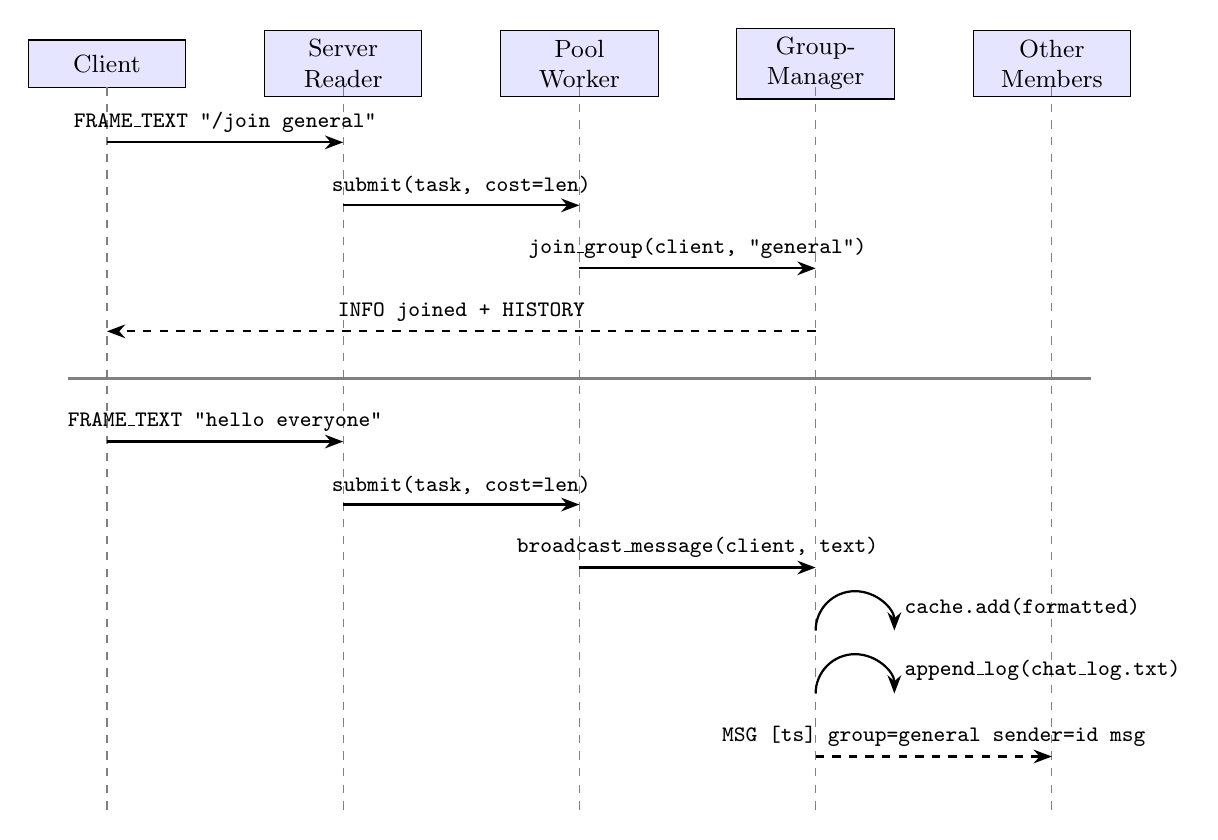
\begin{tikzpicture}[
    actor/.style={rectangle, draw, fill=blue!10, minimum width=2.0cm,
                  minimum height=0.6cm, align=center, font=\small},
    msg/.style={-Stealth, thick},
    retmsg/.style={-Stealth, dashed, thick},
    note/.style={font=\footnotesize\ttfamily}
  ]

  % Actors (lifeline headers)
  \node[actor] (C)  at (0,0)    {Client};
  \node[actor] (S)  at (3,0)    {Server\\Reader};
  \node[actor] (P)  at (6,0)    {Pool\\Worker};
  \node[actor] (G)  at (9,0)    {Group-\\Manager};
  \node[actor] (O)  at (12,0)   {Other\\Members};

  % Lifelines
  \foreach \x in {0,3,6,9,12}
    \draw[dashed, gray] (\x,-0.3) -- (\x,-9.5);

  % Message 1: C -> S
  \draw[msg] (0,-1.0) -- node[above,note]{FRAME\_TEXT "/join general"} (3,-1.0);
  % Message 2: S -> P
  \draw[msg] (3,-1.8) -- node[above,note]{submit(task, cost=len)} (6,-1.8);
  % Message 3: P -> G
  \draw[msg] (6,-2.6) -- node[above,note]{join\_group(client, "general")} (9,-2.6);
  % Return: G -> C
  \draw[retmsg] (9,-3.4) -- node[above,note]{INFO joined + HISTORY} (0,-3.4);

  \draw[thick, gray] (-0.5,-4.0) -- (12.5,-4.0);

  % Second sequence
  \draw[msg] (0,-4.8) -- node[above,note]{FRAME\_TEXT "hello everyone"} (3,-4.8);
  \draw[msg] (3,-5.6) -- node[above,note]{submit(task, cost=len)} (6,-5.6);
  \draw[msg] (6,-6.4) -- node[above,note]{broadcast\_message(client, text)} (9,-6.4);
  % Self-arrows on G
  \draw[msg] (9,-7.2) arc[start angle=180, end angle=0, radius=0.5cm]
        node[right,note,yshift=0.3cm]{cache.add(formatted)};
  \draw[msg] (9,-8.0) arc[start angle=180, end angle=0, radius=0.5cm]
        node[right,note,yshift=0.3cm]{append\_log(chat\_log.txt)};
  % Broadcast to Others
  \draw[retmsg] (9,-8.8) -- node[above,note]{MSG [ts] group=general sender=id msg} (12,-8.8);
\end{tikzpicture}
\caption{Sequence diagram: client join and text message flow through the system.}
\end{figure}

% ============================================================
\section{Message Protocol Design}

\subsection{Existing Transport Frame}

The current implementation uses a compact transport frame:

\begin{itemize}[leftmargin=1.5em]
  \item 1 byte: frame type
  \item 4 bytes: payload size
  \item N bytes: payload bytes
\end{itemize}

This supports both text and binary media chunks.

\subsection{Assignment Packet Format (Required Fields)}

To satisfy the required packet design fields (\texttt{type}, \texttt{group ID},
\texttt{timestamp}, \texttt{payload size}, \texttt{payload}), the project defines
the following logical packet header for chat/media messages:

\begin{lstlisting}[style=cstyle, caption={MessagePacketHeader --- network byte order (big-endian)}]
// Network byte order (big-endian)
struct MessagePacketHeader {
  uint8_t  type;         // chat, join, leave, audio chunk, video chunk, etc.
  uint32_t group_id;     // numeric group identifier
  uint64_t timestamp_ms; // Unix epoch time in milliseconds
  uint32_t payload_size; // number of bytes following header
};
// uint8_t payload[payload_size];
\end{lstlisting}

\medskip
\noindent\textbf{Field semantics:}
\begin{itemize}[leftmargin=1.5em]
  \item \texttt{type}: protocol operation code.
  \item \texttt{group\_id}: routes message to exactly one logical group.
  \item \texttt{timestamp\_ms}: server or sender time metadata used for ordering/logging.
  \item \texttt{payload\_size}: bounds checking and allocation safety.
  \item \texttt{payload}: UTF-8 text bytes or raw binary media bytes.
\end{itemize}

\subsection{Type Values}

\begin{center}
\begin{tabular}{ll}
\toprule
\textbf{Value} & \textbf{Meaning} \\
\midrule
\texttt{0x01} & text chat \\
\texttt{0x02} & join group \\
\texttt{0x03} & leave group \\
\texttt{0x04} & audio begin \\
\texttt{0x05} & audio chunk \\
\texttt{0x06} & audio end \\
\texttt{0x07} & video begin \\
\texttt{0x08} & video chunk \\
\texttt{0x09} & video end \\
\texttt{0x0A} & server info/error \\
\bottomrule
\end{tabular}
\end{center}

\subsection{Validation and Robustness Rules}

\begin{itemize}[leftmargin=1.5em]
  \item Reject packets where \texttt{payload\_size > MAX\_FRAME\_SIZE}.
  \item Sanitize filenames before media forwarding.
  \item Reject text/media attempts if sender is not in a group.
  \item Treat unknown \texttt{type} values as protocol errors.
\end{itemize}

% ============================================================
\section{Cache Design}

\subsection{Cache Size and Eviction Policy}

Each chat group owns a fixed-size message cache of 20 entries.

\begin{itemize}[leftmargin=1.5em]
  \item \textbf{Capacity:} 20 messages per group.
  \item \textbf{Effective policy:} circular/FIFO eviction (oldest dropped first).
  \item \textbf{Data structure:} deque-like container for O(1) append and pop-front.
\end{itemize}

\medskip
\noindent\textit{Note on terminology:} The assignment allows LRU or Circular.
This implementation uses Circular FIFO, which is simpler and deterministic for
recent-history replay.

\subsection{Storage and Retrieval}

\noindent\textbf{Storage path:}
\begin{enumerate}[leftmargin=1.5em]
  \item Worker formats outgoing message with timestamp, group, sender.
  \item Group cache appends formatted string.
  \item If full, oldest entry is evicted.
  \item Message is also appended to persistent log file.
\end{enumerate}

\noindent\textbf{Retrieval path:}
\begin{enumerate}[leftmargin=1.5em]
  \item Client joins a group.
  \item Server loads that group's in-memory history snapshot.
  \item Server sends \texttt{HISTORY} lines to the joining client in chronological order.
\end{enumerate}

\subsection{Synchronization Approach}

Group data is shared mutable state, protected by one mutex in \texttt{GroupManager}.

\medskip
\noindent\textbf{Critical sections cover:}
\begin{itemize}[leftmargin=1.5em]
  \item \texttt{groups\_} membership and per-group cache updates.
  \item \texttt{client\_group\_} membership map.
  \item \texttt{client\_ids\_} sender identity map.
\end{itemize}

\noindent\textbf{Thread pool synchronization:}
\begin{itemize}[leftmargin=1.5em]
  \item Internal queue lock for enqueue/dequeue operations.
  \item \texttt{condition\_variable} used to sleep idle workers and wake them on submit.
\end{itemize}

\noindent\textbf{Concurrency safety goal:}
\begin{itemize}[leftmargin=1.5em]
  \item No concurrent unsynchronized writes to membership/cache structures.
  \item No busy-waiting in worker threads.
\end{itemize}

% ============================================================
\section{Scheduling Design}

\subsection{Strategy}

The server supports two dispatch strategies for text tasks:

\begin{itemize}[leftmargin=1.5em]
  \item \textbf{RR (Round Robin / FIFO queue):} first submitted, first executed.
  \item \textbf{SJF (Shortest Job First):} smallest \texttt{cost} first,
        where cost is message length in bytes.
\end{itemize}

\medskip
\noindent\textbf{Educational value:}
\begin{itemize}[leftmargin=1.5em]
  \item RR demonstrates fairness and predictable order.
  \item SJF demonstrates throughput optimization for short jobs.
  \item Both are implemented at application level on top of OS thread scheduling.
\end{itemize}

\subsection{Task Dispatch Queue Diagram}

\begin{figure}[H]
\centering
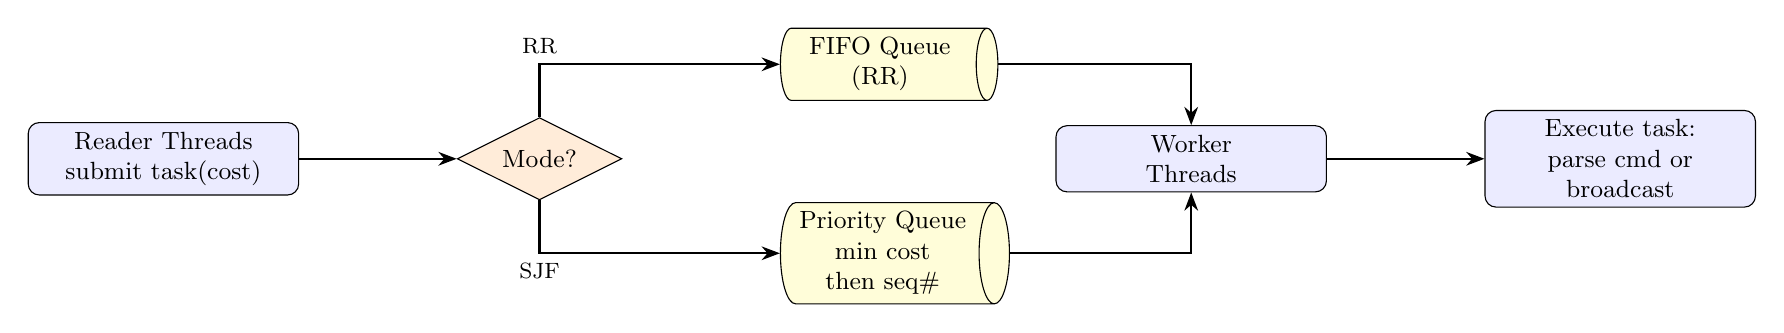
\begin{tikzpicture}[node distance=1.2cm and 2.2cm]
  \node[block] (in) {Reader Threads\\submit task(cost)};
  \node[decision, right=2.0cm of in] (sel) {Mode?};
  \node[dbblock, right=2.0cm of sel, yshift=1.2cm] (rr) {FIFO Queue\\(RR)};
  \node[dbblock, right=2.0cm of sel, yshift=-1.2cm] (sjf) {Priority Queue\\min cost\\then seq\#};
  \node[block, right=5.5cm of sel] (w) {Worker\\Threads};
  \node[block, right=2.0cm of w] (exec) {Execute task:\\parse cmd or\\broadcast};

  \draw[arrow] (in) -- (sel);
  \draw[arrow] (sel.north) |- node[above,font=\footnotesize]{RR} (rr.west);
  \draw[arrow] (sel.south) |- node[below,font=\footnotesize]{SJF} (sjf.west);
  \draw[arrow] (rr.east) -| (w.north);
  \draw[arrow] (sjf.east) -| (w.south);
  \draw[arrow] (w) -- (exec);
\end{tikzpicture}
\caption{Task dispatch queue: RR uses a plain FIFO; SJF uses a min-priority queue
         keyed on (cost, sequence).}
\end{figure}

\subsection{Dispatch Rules}

\begin{itemize}[leftmargin=1.5em]
  \item Every text line becomes one task with \texttt{cost = line.length}.
  \item SJF tie-breaker uses a monotonically increasing sequence number to preserve
        stable ordering among equal-cost tasks.
  \item Media frames are relayed immediately by reader threads and are \emph{not}
        pooled as text tasks.
\end{itemize}

% ============================================================
\section{Extra Features Plan (Optional)}

\subsection{Audio/Video Simulation Plan}

\noindent\textbf{Current status:}
\begin{itemize}[leftmargin=1.5em]
  \item Supports \texttt{/audio <path>} and \texttt{/video <path>} commands.
  \item Uses begin/chunk/end framing for streaming-like transfer.
  \item Clients can play last or specified file with \texttt{/play [path]}.
\end{itemize}

\noindent\textbf{Planned enhancements:}
\begin{itemize}[leftmargin=1.5em]
  \item Add progress feedback per transfer (percent + bytes).
  \item Add configurable chunk sizes based on runtime bandwidth.
  \item Add transfer interruption/retry support.
\end{itemize}

\subsection{Client Verification Logic Plan}

\noindent\textbf{Current baseline checks:}
\begin{itemize}[leftmargin=1.5em]
  \item Must join a group before sending media.
  \item Server rejects unknown/invalid commands in chat path.
  \item Filenames are sanitized before use.
\end{itemize}

\noindent\textbf{Planned verification improvements:}
\begin{itemize}[leftmargin=1.5em]
  \item Add client handshake with protocol version.
  \item Enforce maximum command length and UTF-8 validity for text payloads.
  \item Add per-client rate limiting for spam/flood protection.
\end{itemize}

\subsection{Security/Permissions Plan}

\noindent\textbf{Current state:}
\begin{itemize}[leftmargin=1.5em]
  \item Basic input sanitation and bounded frame sizes.
  \item Group membership constrains media/message fan-out.
\end{itemize}

\noindent\textbf{Planned security extensions:}
\begin{itemize}[leftmargin=1.5em]
  \item Group access control lists (private/public groups).
  \item Role model (\texttt{owner}, \texttt{moderator}, \texttt{member}) with command permissions.
  \item Optional authentication token at connection setup.
  \item Structured audit log for joins/leaves/admin actions.
\end{itemize}

% ============================================================
\section{Summary}

This design provides a complete OS-focused chat architecture with:

\begin{itemize}[leftmargin=1.5em]
  \item Real concurrency (client reader threads + worker thread pool).
  \item Explicit scheduling policy control (RR and SJF).
  \item Bounded in-memory cache with deterministic eviction.
  \item A binary packet header design covering all required fields.
  \item Optional extension path for media quality, verification, and security.
\end{itemize}

\medskip
\noindent The document can be submitted directly as the project design report.

\end{document}
